% Created 2022-10-21 Fri 18:49
% Intended LaTeX compiler: pdflatex
\documentclass[hidelinks,11pt]{article} \usepackage[utf8]{inputenc}
\usepackage[T1]{fontenc} \usepackage{graphicx} \usepackage{longtable}
\usepackage{wrapfig} \usepackage{rotating} \usepackage[normalem]{ulem}
\usepackage{amsmath} \usepackage{amssymb} \usepackage{capt-of}
\usepackage{hyperref} \usepackage{caption}
\usepackage{subcaption} % sufigures facilities
\usepackage{float} % for H option
\usepackage{xcolor} % for the textcolor command
\usepackage[a4paper,width=150mm,top=25mm,bottom=25mm]{geometry} % fixes margins
\usepackage{changepage} \author{Marcelo Veloso Maciel\thanks{I thank Marek
    Kaminski, Donald Saari, and Ines Levin for their guidance and encouragement,
    and Maria Luiza Paschoal, Kaique Pereira Santos, John Brunson, Udita Ghosh
    and Joshua Storm for their feedback on this project.}} \date{}

\title{Majoritarian principles and critical junctures: an analysis of Brazil's
  2018 presidential election}

\hypersetup{
 pdfauthor={Marcelo Veloso Maciel},
 pdftitle={W4 Essay},
 pdfkeywords={},
 pdfsubject={},
 pdfcreator={Emacs 28.2 (Org mode 9.6)},
 pdflang={English}}
\usepackage[authordate,strict,backend=biber,
bibencoding=inputenc]{biblatex-chicago}
%\setlength{\textfloatsep}{0.1cm}
\addbibresource{refs.bib}
\begin{document}

\maketitle
\begin{abstract}
  Presidential Elections are critical moments for polyarchical systems,
  particularly in contexts of high social tension. The 2018 presidential
  election in Brazil used a two-round system, yet the most divisive candidates
  went to the second round. Pairwise and positional voting procedures embody
  different generalizations of a majoritarian credo that underpins such
  elections. The paper mobilizes both perspectives and, using representative
  survey data, reconstructs the top four preferences of the Brazilian electorate
  a week before the election. It shows that the electoral winner, Jair Messias
  Bolsonaro, was a Condorcet Winner, but may have not been the Borda Winner,
  while the second-round loser, Fernando Haddad, was a Condorcet Loser.
  Furthermore, possible alternative scenarios under different feasible sets of
  candidates are simulated, contributing to understanding the role of decision
  procedures in critical junctures.
  \end{abstract}
% parencite for indirect citation, textcite for direct citation
\section{Introduction}

The rise of polarization, the specter of democratic backsliding, and more
generally an apprehension with the survival prospects of democratic polities\footnote{For a critical perspective on the current academic discourse on democratic backsliding see \textcite{little2023subjective}.}
have led to a renewed interest in what institutions mitigate vs. instigate
destabilizing dynamics, or that increase the adaptability of the political
system vis-\`a-vis both internal and external stressors
\parencite{Bednare2113843118, chiopris2021wolf, tarko2014institutional, ostrom1997meaning}. Given
their centrality to the input-output relation between society and the state,
electoral institutions naturally figure among the set of such institutions under
scrutiny \parencite{Wange2021systems}, and a branch of the literature on
collective choice has wondered whether the current electoral victories of
divisive candidates have not been an effect of informationally poor decision
procedures \parencite{potthoff2021condorcet, kurrild2018trump, woon2020trump}.
This paper shows, however, that in 2018 presidential election in Brazil the
election of a polarizing candidate, Jair Messias Bolsonaro, was not simply an
artifact of the decision procedure. Despite that, neither would he have won
under any reasonable voting method. I demonstrate that, in this case, there is a
partial conflict between typical evaluative positions, harking back to the Borda-Condorcet debate.

Despite the multiple historical contingencies that might explain his victory,
one might naturally wonder what role the electoral system has had in it. After
all, it is well-known that the outcome of collective choices is fundamentally
dependent on the voting procedure \parencite{riker1982liberalism}. As Brazil's
two-round system, most electoral systems merely use the first index of the
voters' preference rankings \parencite{grofman04_if_you_like_alter_vote}. How
would he have fared under informationally richer voting procedures, such as
methods based on pairwise comparisons and positional voting procedures? Was he,
and arguably other democratically elected destabilizing candidates, a product of
decision procedures that favor divisive candidates over more inclusive ones
\parencite{igersheim22_compar_votin_method}? What criteria should be used to
argue that a candidate's victory was an institutional artifact? Would the result
have changed with a different set of candidates?

To answer those questions, I, first, revisit the perspectives of Borda and
Condorcet on voting procedures. After that, I use a pre-electoral representative
survey to reconstruct the full 4-top rankings of the Brazilian population and
use this augmented data to simulate electoral outcomes, under alternative
methods, for the top 4 and 3 candidate sets. Finally, I discuss the significance
of the results and conclude by pointing out the limitations of this endeavor.

\section{Theory}

The realization that the result of collective decisions is inseparable from the
voting procedures being used and that such procedures differ in terms of their
consistency with evaluative criteria naturally leads us to wonder what possible
adjacent paths could have been taken in key electoral moments
\parencite{tabarrok1999would, kaminski1999communism, ostrom1986agenda}.
Concurrently, this realization puts us in a conundrum: what, among all possible
criteria, should be used to motivate the counterfactual analysis? Isn't this
endeavor inherently arbitrary, given that one can always retrofit a choice of
voting method that matches an a-priori desired outcome
\parencite{riker1982liberalism}? The anchoring point is to note that political
actors themselves reflect on those procedural properties, which end up being
levers for their legitimacy claims within the political game
\parencite{mclean02_william_h, ostrom2009understanding}. Thus, rather than
assuming a philosopher-king stance and imposing external values as if they were
universally agreeable, we can look at what set of values the agents themselves
mobilize \parencite{binmore2005natural}. Particularly prominent among polarizing
or divisive candidates -those that have strong support at the top choices of
voters, but also have a high share of the bottom choices among the
electorate\footnote{The correspondent concept of an inclusive candidate is
  defined by \textcite[p.6]{igersheim22_compar_votin_method} as those that
  ``get widespread support from the voters but with no strong feeling of
  rejection or attachment''.}- are claims of strength and legitimacy based on
the notion of popular mandate, a congenial resource for politicians that,
despite being elected, face widespread rejection or opposition.


Nevertheless, what is a mandate? At a minimum, a politician has a mandate as
long as he has won under the voting procedure. An actor has more mandate the
more significant the difference between its vote share or score vs. the second
most well-voted candidate. Such an agent has more marginal mandate rather than
just having the minimal mandate bestowed by winning. Note that both notions of
the mandate are related to a fundamental majoritarian credo which is part of the
democratic ideal: that if both alternatives and voters are deemed equals, then
the alternative that receives more support should be the winner
\parencite{dahl1989democracy}. This ``monotonic/majoritarian mindset'' underlies
the minimal mandate, since if a candidate was elected, it received more votes
than the others, and the stronger marginal mandate, since more support means
more mandate. That majoritarian value is what sustains claims of legitimacy of
elected candidates. Roughly, the higher the marginal mandate, the more backing
of popular support an Executive leader can claim to have
\parencite{grossman2022majoritarian}. Alternatively, to deny the opposition has
achieved a mandate by claiming the electoral process is fraudulent is a maneuver
that again mobilizes this focal point of the democratic ethos.

However, with more than 2 alternatives, the majoritarian mindset is not as
clear-cut as a profile, voters' rankings, such as [xyz, yzx, zxy] reminds us.
Nonetheless, it remains a centerpiece of the democratic paradigm. How can, then,
one extend majoritarianism to more than two alternatives? Borda and Condorcet
grappled with this problem and gave different answers. Condorcet extended the
majority rule to pairwise majority rule: apply majority rule to all pairwise
comparisons. One possible condition that generalizes majoritarianism is what is
known as the Condorcet criterion: a decision procedure is Condorcet consistent
if it selects the candidate, if there is any, that wins in all pairwise majority
contests. This alternative is called a Condorcet winner (CW)
\parencite{felsenthal2011review}. Borda, on the other hand, devised a scoring
scheme: if there are say 3 alternatives \(\{A,B,C\}\) and an agent \(i\) has
ranking \(B>C>A\) then the Borda score in \(i\)'s ranking for each alternative
is \(A:B:C = 0:2:1\)\footnote{Alternatively, it can also be coded as
  \(1:3:2\).}. The Borda score for the full profile is the sum of each
alternative score at each voter ranking, and the candidate with the highest
score, the Borda winner (BW), wins. It is equivalent to adding the number of
votes an alternative got in each pairwise comparison against the other
alternatives \parencite{nurmi1999voting}. As such, it is another way of
generalizing the ``majoritarian/monotonic'' perspective to more than two
alternatives.

Being Condorcet consistent is arguably the primary normative benchmark for a
voting method in single-candidate elections, while the Borda perspective could
be considered the leading contender \parencite{regenwetter2006behavioral,
  felsenthal2011review, nurmi2002voting}. While being plausible generalizations
of the majoritarian credo, they also offer stronger and informationally more
demanding views of mandate. If the candidate is a CW, it would have won under
all possible majority pairwise comparisons against the other candidates. I will
say a CW is a candidate with pairwise mandate\footnote{The Copeland scores could
  be a more general measure of pairwise mandate or even the Kemeny scores for
  each permutation, but this generalization is unnecessary in the context of
  this paper.}. The BW lends itself to a similar interpretation, but the notion
of mandate can be strengthened here. The Borda count can be seen as one method
within a family of methods that assign weights to positions in the ballot. In
one extreme, the plurality voting method assigns a score of 1 to the top choice
and 0 to all others. On the other extreme is the antiplurality voting method,
which assigns 1 to all positions besides the last one. Between the two extremes
are all possible ways of assigning a score to the ballots of the electorate. The
higher the proportion of positional voting systems that the candidate would have
won had the election used it, what \textcite{tabarrok2001president} has called
positional stability, the higher the positional mandate of the candidate.

Suppose a candidate wins under a voting procedure that only uses the top choice
of the electorate but is neither a BW nor a CW. In that case, it has less
mandate, in this generalized majoritarian perspective, than if it were both -
which would signal a comprehensive social basis. Thus, a candidate who wins
under the current voting procedure but is neither a BW nor a CW could be
considered an artifact of the procedure. In the latter case, the procedure would
be just ``tracking'' a broader support pattern for the alternative. Altogether,
the notions of pairwise and positional mandates will be the primary lenses in
this paper to understand both the popular support a candidate receives and the
role of the decision procedure in its election.

Even though the pairwise and positional perspectives of popular support/mandate
generalize a widely held democratic principle, they are not captured by
electoral processes that only have as input voters' first choice. As such, they
are not typically mobilized by politicians. Nonetheless, this information, which
has been repeatedly rediscovered in acts of political reflexivity
\parencite{mclean14_stran_histor_social_choic_contr}, can be queried to tell a
more refined story about the backing a candidate has among the electorate. Such
a broader informational backdrop underlies current research on the case of the
United States and Donald Trump's electoral victory. Regardless of the
specificities of each paper, all presuppose that the informational paucity of
only focusing on top choices blinds the States' socio-technical translation of
popular support into political input (the choice of a candidate). For instance,
\textcite{potthoff2021condorcet, woon2020trump, kurrild2018trump} debate whether
Donald Trump was a CW in the primaries, with recommendations of voting
procedures that better track what the CW is, after all.
\textcite{igersheim22_compar_votin_method} goes a step further: they argue that
not only was Trump neither, but Sanders was the actual Borda and Condorcet
Winner, and generally the ``best'' candidate, if by best one understand a
candidate being the most inclusive and winning under the most alternative
decision procedures\footnote{I doubt this distribution of support for Sanders
  would hold had he been a viable candidate.}. An analogous line of reasoning
would lead us to hypothesize that a similar conclusion could be drawn about
Bolsonaro: he would not have either pairwise or positional mandate. We will see,
however, that an unambiguous conclusion cannot be drawn in the Brazilian case.

\section{Case/Data}

Jair Messias Bolsonaro was elected the president of Brazil in 2018. For more
than 20 years as a congressman, he was primarily a low clergy politician
defending the interests of the military and local police forces of the state of
Rio de Janeiro. The 2018 electoral scenario in Brazil was one of high rejection
of the traditional political elite, particularly of the Labor Party (Partido dos
Trabalhadores - PT), after corruption scandals and an impeachment process of the
previous president, Dilma Roussef, a Labor politician.


The main contestants, among 13, were him, a rightist candidate; Fernando Haddad,
a leftist candidate from PT; Geraldo Alckmin, a center-right candidate; and Ciro
Gomes, a center-left candidate. The presidential election in Brazil follows a
two-round system. In the first round, \(8.79\%\) of the votes were White/Null,
which means the voting procedure does not count them. Moreover, there was a
\(20\%\) abstention. The result of the valid votes was, in percentages, the
following: Bolsonaro:Haddad:Ciro:Alckmin:Others =
\(46.3:29.28:12.47:4.76:7.19 \). Among the 9 other candidates, the highest vote
share was Jo{\~a}o Amo{\^e}do's with \(2.5\%\). All others got less than
\(1\%\). In the second round, the result was: Bolsonaro:Haddad =
\(55.12 : 44.78 \). White/Null votes were \(9.57\%\) of the total electorate.
The abstention in this round was \(21.3\%\). With more than \(10\%\) more than
his second-round opponent, Bolsonaro rose to power backed by a solid marginal
mandate. Nevertheless, he still contested the result and argued that he would
have won in the first round had the elections not been frauded\footnote{No
  evidence has been found of any rigging of the elections in Brazil, despite his
  claims.}. He continued putting the electoral institutions under suspicion with
a view to the 2022 election, which he lost to Lula with a margin of \(1\%\).


It is relevant to notice that two events marked the 2018 election. First, the
leading leftist candidate, Lula, was prevented from running. He was arrested at
the beginning of the electoral campaigns, the process was deemed suspicious in
2021 since the judge\footnote{Bolsonaro nominated this judge Minister of
Justice.} was cooperating with the prosecutor, and he won in 2022, in an
electoral process marked by irregularities in favor of Bolsonaro. The
distribution of support for Lula was markedly different from Haddad, who was
merely his replacement. PT's campaign was predicated on the possibility of Lula
being released, and Haddad posed primarily as Lula's candidate. Nonetheless, his
popularity was nowhere near Lula's, and he inherited the high rejection of his
party at the time. Second, on 09/06/2018, a month before the first round, there
was an assassination attempt against Bolsonaro. The knife attack most likely
changed his pattern of support.

The dataset used for the analysis is a representative street survey done on
10/02/2018, less than a week before the first round (10/07/2018). DataFolha, an
independent research institute highly esteemed and trusted by Brazilian
experts\footnote{I had access to the survey data, code-book, and questionnaire
by creating an account and requesting access to them, available for
educational/research purposes, at \url{https://www.cesop.unicamp.br}.}, did this
survey. One question, in particular, is the only variable in our analysis:
pairwise comparisons between the 4 top candidates. With it is possible to
reconstruct the full 4-top ranking of the voter. Preliminary pre-processing has
led me to drop 171 observations where all pairwise comparisons were missing and
132 in which they were cyclic. This leaves us with 2937 out of 3240
observations. As Table~\ref{Tab:Tcpairwise} shows only 1797 observations
compared all 4 candidates. As such, we have to augment the data with transitive
closures for 1140 observations by methods discussed in the next section.

\begin{table}[]\centering \resizebox{0.5\columnwidth}{!}{
\begin{tabular}{|l|r|} \hline Number of Pairwise Comparisons & Frequency \\
\hline 1 & 15 \\ \hline 2 & 42 \\ \hline 3 & 462 \\ \hline 4 & 118 \\ \hline 5 &
503 \\ \hline 6 & 1797 \\ \hline
\end{tabular} }
\caption{Frequency of pairwise comparisons in the dataset.}

\label{Tab:Tcpairwise}
\end{table}


\section{Methods}

I impute the missing data using the \textbf{\textsf{R}} package
\(\operatorname{mice}\) (multiple imputation by chained equations), one of the
standard packages for this task. It fills the missing values in a row by using
the values of the other columns, by an iterative series of predictive models
\parencite{vanbuuren2018imputation}. Under the hood, it offers a menu of
possible predictive models, such as bayesian linear regression, predictive mean
matching, logistic regression, polytomous regression, classification trees and
random forests. Among the classes of methods that could be applied to the
missing voting data, given its categorical nature, the polytomous regression was
the only one that did not introduce cyclic rankings, or repeated alternatives in
the ranking, and as such, was the one I used\footnote{Besides the polytomous
regression, I tested predictive mean matching, classification trees, and random
forests. All introduced cyclic rankings, sometimes in large amounts (as in the
case of random forests).}.

A further complication is a mismatch between the survey's plurality result and
the actual result of the first round. This is typical in surveys and might be
due to strategic voting, social desirability bias (not wanting to be seen as
``extreme''), or systematic refusal of part of the electorate to answer the
survey \parencite{nishimura2016alternative}. Any imputation technique will
reproduce this top-choice discrepancy since it inherits this problem from the
survey. The share in the survey is Bolsonaro:Haddad:Ciro:Alckmin:Others =
\(36.81 : 24.96 : 17.06: 13.97 : 7.2 \). Thus, Bolsonaro and Haddad are
undervoted in the sample, while Ciro and Alckmin are overvoted\footnote{Remember
the actual result was Bolsonaro:Haddad:Ciro:Alckmin:Others =
\(46.3 : 29.28 : 12.47 : 4.76 : 7.19 \).}. However, transferring is complicated
by the fact that we are working with the full rankings, which gives leeway to
many possible ways of transferring. For instance, consider Table
~\ref{tbl:overunderex}, which shows some of the rankings for Alckmin and
Bolsonaro after the imputation. If we are to transfer from Alckmin to Bolsonaro,
we are led to the problem of first picking which ranking at the source should be
chosen and then which ranking at the target should receive votes while
respecting how much the source has in excess and how much the target needs.
Which row from the set \(\{1,2,3\}\) should transfer votes to which row of the
set \(\{4,5,6\}\)?

\begin{table}[!h] \centering %\resizebox{0.8\columnwidth}{!}{
\begin{tabular}{rllllrr} \hline & 1 & 2 & 3 & 4 & frequency & proportion \\
\hline 1 & Alckmin & Bolsonaro & Ciro & Haddad & 93 & 0.03 \\ 2 & Alckmin & Ciro
& Bolsonaro & Haddad & 63 & 0.02 \\ 3 & Alckmin & Haddad & Bolsonaro & Ciro & 14
& 0.00 \\ 4 & Bolsonaro & Alckmin & Ciro & Haddad & 556 & 0.18 \\ 5 & Bolsonaro
& Ciro & Alckmin & Haddad & 366 & 0.12 \\ 6 & Bolsonaro & Alckmin & Haddad &
Ciro & 59 & 0.02 \\ \hline
\end{tabular} %}
\caption{Some pre-transfer proportions of Alckmin/Bolsonaro's rankings}
\label{tbl:overunderex}
\end{table}

A natural sorting of which ranking should be the source is the position
Bolsonaro is in the ranking. We start with rankings in which he is in the second
position ((Alckmin, Bolsonaro, Ciro, Haddad), (Alckmin, Bolsonaro, Haddad,
Ciro)), then third position ((Alckmin, Ciro, Bolsonaro, Haddad), (Alckmin,
Haddad, Bolsonaro, Ciro )), then last position ((Alckmin, Ciro, Haddad,
Bolsonaro), ((Alckmin, Haddad, Ciro, Bolsonaro))).

Suppose we picked a source ranking from the first sorted rankings set. What
should be the target ranking among the rankings which have Bolsonaro as the
first choice? I transfer to the ranking that has minimal Kemeny's distance to
the source ranking \parencite{nurmi2002voting}. The Kemeny distance counts the
number of transpositions (switching of pairs) needed to go from one permutation
to another permutation. Thus, I transfer from the source ranking the
\(\operatorname{\mathbf{min}}\)(number of votes the source ranking has, the
total number of votes the under-voted needs, the total number of votes the
over-voted can give)\footnote{The \(\operatorname{\mathbf{min}}\) guarantees: we
are not giving more than the source ranking has, which would lead to negative
numbers; less or more than the undervoted needs; nor giving more than the
over-voted should overall give (at some iteration in the loop, a ranking can
have a higher frequency than both what the over-voted can give and the
under-vote needs to receive).}. I update the source ranking frequency, the
target ranking frequency, the total number of votes the under-voted needs, and
the total number of votes the over-voted can give. If the under-voted does not
need any other votes, the algorithm breaks the loop and goes to another
over-voted \(\to\) under-voted transfer. If not, it checks if the over-voted can
still transfer votes to the current target under-voted. If yes, it picks another
source ranking in the sorted rankings sets and repeats until the source has run
out of votes it can give or the target has received enough votes. If not, it
goes to another over-voted \(\to\) under-voted transfer. In the end, this leads
to 24 possible transfer sequences from over-voted to under-voted. One possible
sequence is Alckmin \(\to\) Bolsonaro, then Alckmin \(\to\) Haddad, then Ciro
\(\to\) Haddad, then Ciro \(\to\) Bolsonaro. Another possible sequence is
Alckmin \(\to\) Bolsonaro, then Alckmin \(\to\) Haddad, then Ciro \(\to\)
Bolsonaro, then Ciro \(\to\) Haddad. That transference process leads to 6
transfers that minimize the Euclidean distance between the inferred plurality
result and the actual result of the first round. The results are invariant
between them, so I only report the analysis for one of them. The new percentages
are: Bolsonaro:Haddad:Ciro:Alckmin:Others = \(46.32:29.26:12.45:4.77:7.19 \).

After imputing the missing rankings and making the transfer of rankings to match
the result for the first round, I identify the BW and CW among the top 4
candidates, calculate and plot all counterfactual victory scenarios for
positional voting methods, and visualize the positional outcomes for alternative
3-candidates sets using Saari's outcome simplex \parencite{saari1995basic}.


\begin{figure}[H] \centering 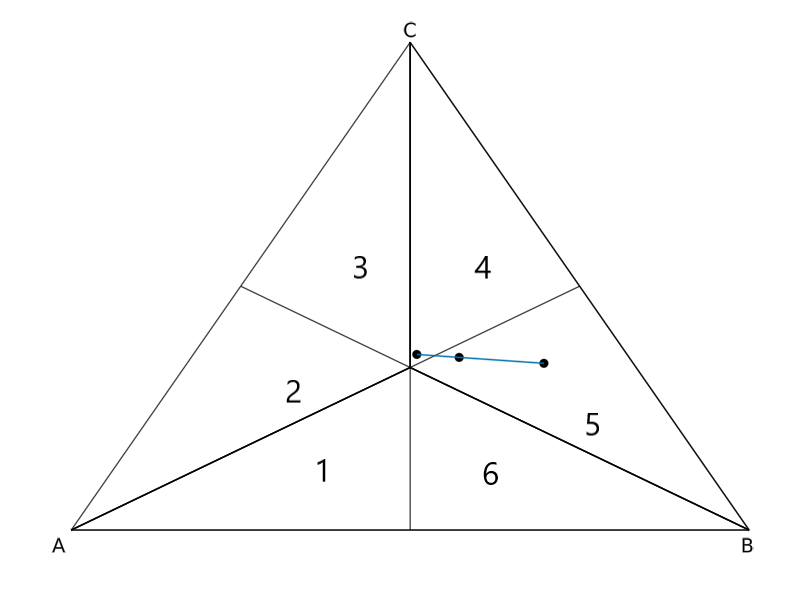
\includegraphics[width=0.8\columnwidth,
height=0.3\textheight]{./images/simpletriangle.png}
 \caption{Saari's outcome simplex}
 \label{fig:saari_nurmi}
\end{figure}

Saari's outcome simplex, or point-share triangle
\parencite{eggers20_diagr_analy_ordin_votin_system}, provides a way of
visualizing all possible positional voting results of an election\footnote{For a
complete exposition of this method see \textcite{saari1995basic} or
\textcite{nurmi2002voting}.}. Consider Figure \ref{fig:saari_nurmi}. The closer
to a vertex, the better the vertex's position in the social ranking. Region 1
corresponds to the social ranking of \(A > B > C\), while Region 4 corresponds
to the social ranking of \(C>B>A\). The lines separating the regions represent
indifference. The point at which all lines meet corresponds to
\(A \sim B \sim C\), while the line separating Region 1 and 2 would correspond
to \(A > B \sim C\). The three dots are the results of the antiplurality, the
Borda and the plurality voting methods. The line connecting the antiplurality
and plurality results, the extremes, denotes all possible positional results,
including the result for the Borda Count. It is called the procedure hull
\parencite{saari2001chaotic}. The Borda Count point is always closer to the
antiplurality result. In this example, most positional voting methods would have
agreed with the plurality procedure outcome of \(B\) as the winner. A related
triangle, the representation triangle, or profile triangle
\parencite{eggers20_diagr_analy_ordin_votin_system}, will be used to represent a
profile compactly. In each ranking region, we plot the frequency of votes that
match that region's ranking. For 4 candidates, we can use analog representations
by ``opening'' the 3-simplex/tetrahedron and plotting onto its polyhedral net -
the arrangement of polyhedrons in the plane that, when folded, become the faces
of the simplex.


To calculate all positional voting victories, I use two facts proved by Donald
Saari \parencite{saari1995basic, saari2001chaotic}: first, any positional voting
method for 4 candidates can be seen as assigning weights to rank positions in a
standardized manner \((1,s_{1},s_{2},0)\), where
\(0 \leq s_{2} \leq s_{1} \leq 1\); second, all such procedures will lie in the
convex hull of the plurality, antiplurality and vote for two procedures, with
respective weights of \((1,0,0,0), (1,1,1,0), (1,1,0,0)\). Calculating scenarios
amounts, thus, to vary the values of \(s_{1}\) and \(s_{2}\).

\section{Results} The inferred rankings are shown in Figure \ref{fig:rep_ot} and
summarized in Figure \ref{fig:counts}. Among all ways of transferring from
over-voted to under-voted, while respecting the Kemeny distance, the
transference that best matched the rankings in the survey with the actual
first-round result led all rankings in which Alckmin appears as the first choice
to be of type Alckmin > Ciro > Haddad > Bolsonaro and Alckmin > Haddad > Ciro >
Bolsonaro. Notably, no ranking of type Alckmin > Bolsonaro > \(\textunderscore\)
> \(\textunderscore\) remained. The most blatant pattern in Figure
\ref{fig:counts} is that the candidates that went to the second round were,
indeed, the most divisive ones. Among the more inclusive candidates, Ciro has
more second choices than third choices, while Alckmin's support is equally
balanced between those two positions in the voters' preferences. Moreover, Ciro
has more first choices and fewer last choices than Alckmin. There is also a
difference among the divisive candidates: Haddad's rejection was higher than his
top-choice support, while the opposite held for Bolsonaro. That within-group,
inclusive vs. divisive, differences will be relevant to understand how each
candidate fares against the others.

\begin{figure}[!h] \centering
  \begin{subfigure}[b]{0.49\textwidth} \centering
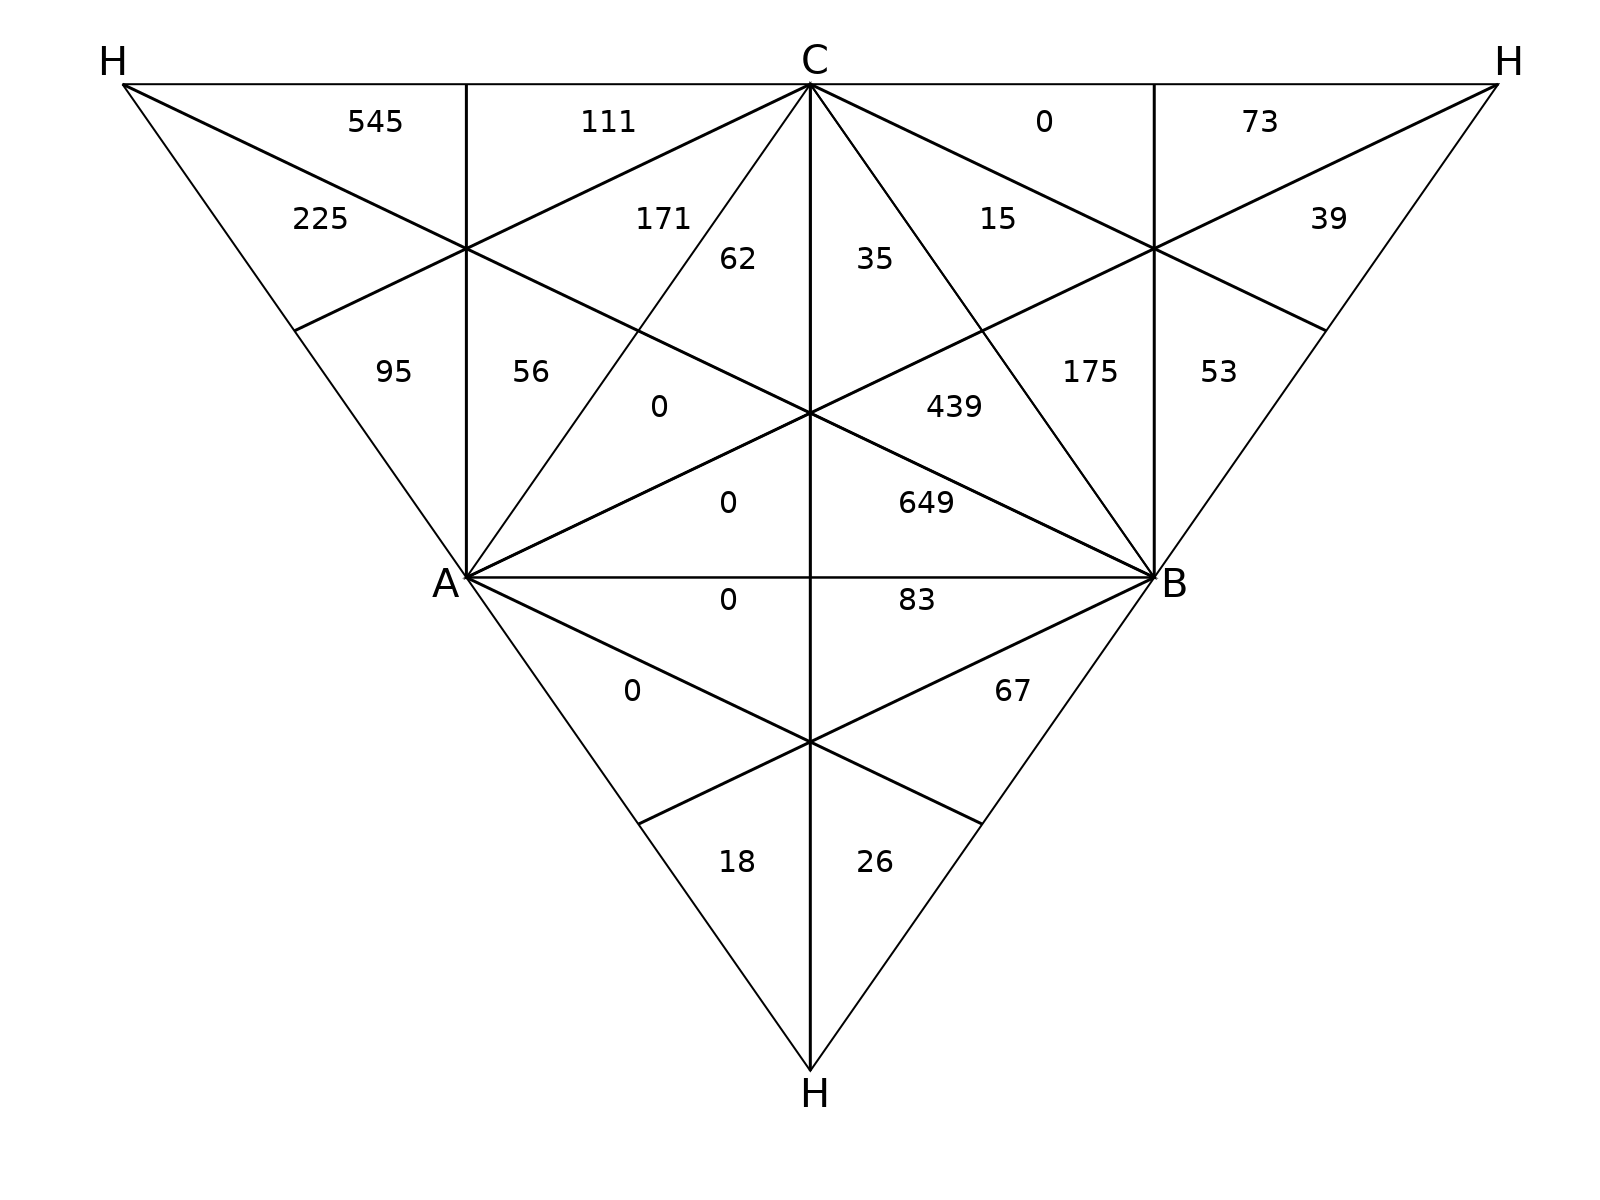
\includegraphics[width=\textwidth]{./images/representation_tetrahedron.png}
 \caption{Opened representation tetrahedron}
 \label{fig:rep_ot}
\end{subfigure} \hfill
  \begin{subfigure}[b]{0.49\textwidth} \centering
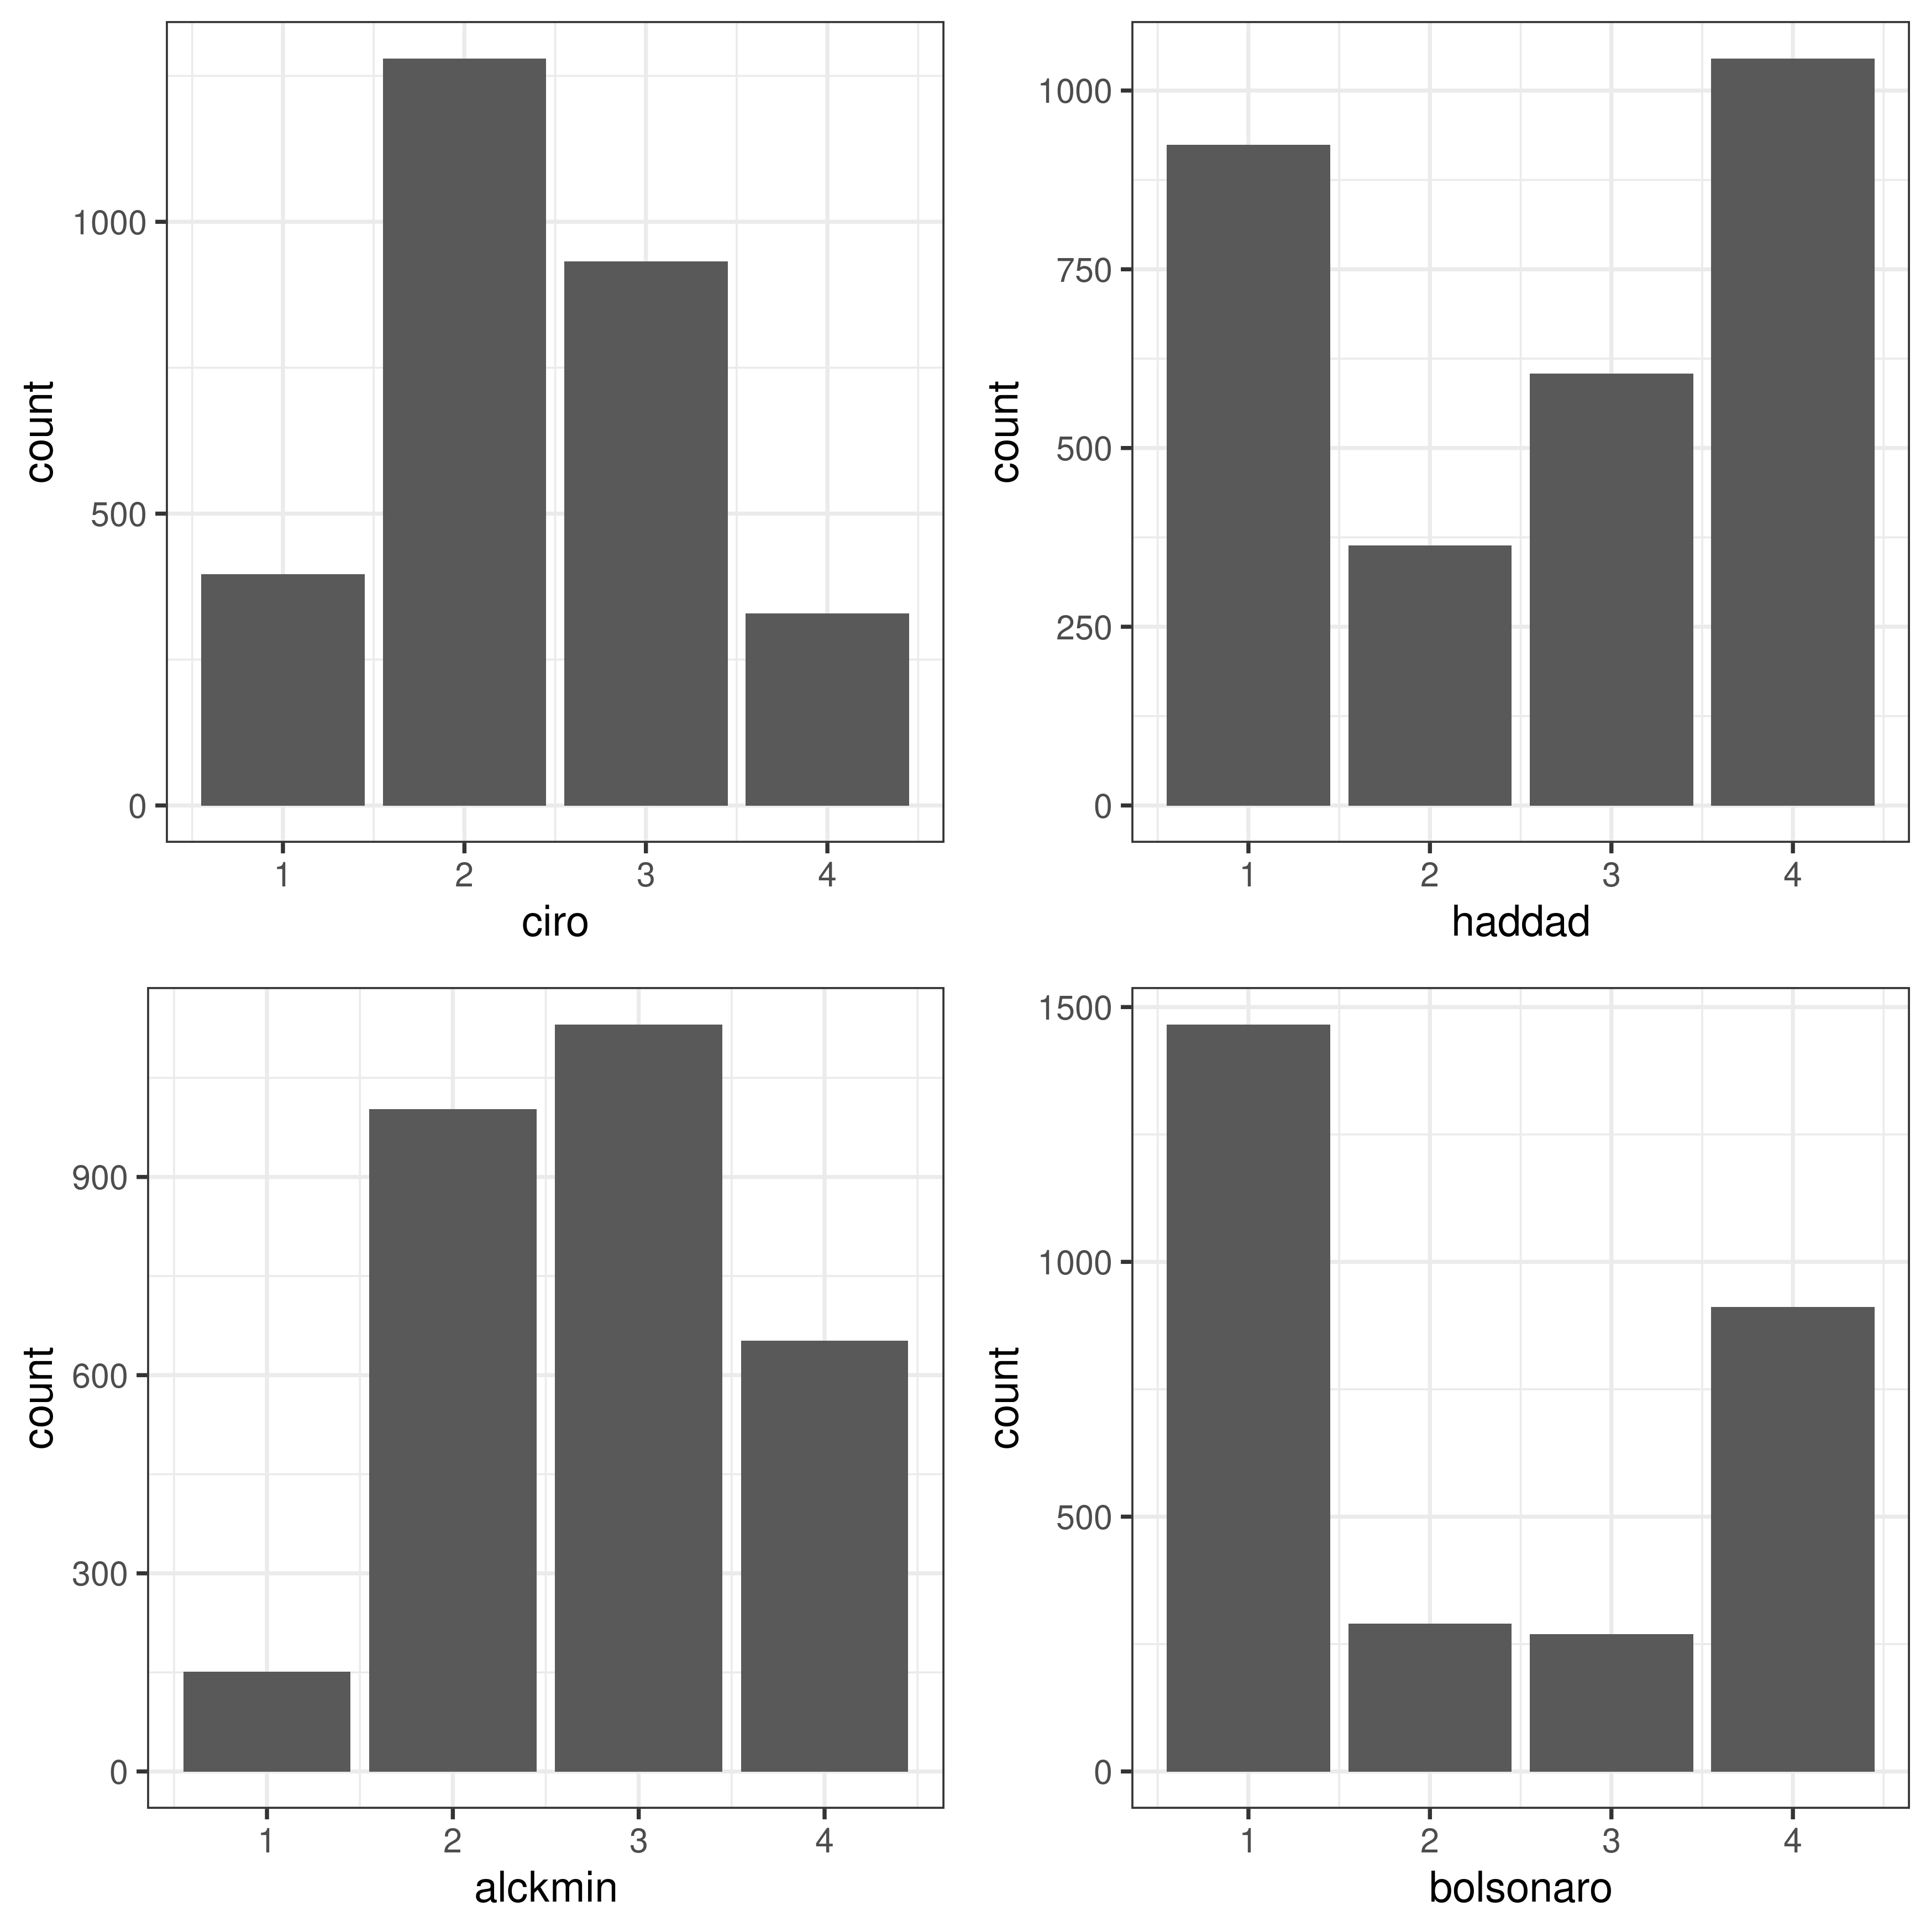
\includegraphics[width=\textwidth]{./images/corrected1_indexes_plot.png}
 \caption{Frequencies at each position}
 \label{fig:counts}
\end{subfigure}
\caption{Profile after imputation and rankings transference}
\label{fig:profile_trans}
\end{figure}

What does this support distribution mean from the point of view of the BW and
CW? Table \ref{tbl:overallresult} shows what we can infer from the imputed data.
Despite being divisive, Bolsonaro would have won in all pairwise majority
comparisons against other top candidates. Haddad, however, would have lost
against all others. He was a Condorcet Loser, despite going to the second round.
Ciro would only have lost against Bolsonaro, while Alckmin could only have won
against Haddad. Unlike what was widely believed at the time and was the motto of
his campaign, it is uncertain whether Ciro would have won against Bolsonaro in
the second round. From a pairwise perspective, he was not the
``anti-Bolsonaro'', but merely an ``anti-Haddad'', even more than Bolsonaro.
Alckmin, the candidate with the longest television time and the broadest
supporting coalition, would have lost against Haddad, who was merely a
substitute for Lula. However, the pattern is not reflected in the Borda Scores,
which implies the ranking: Ciro > Bolsonaro > Alckmin > Haddad. Nevertheless,
the raw Borda scores of Ciro and Bolsonaro are very similar. If we standardize
them, we see that the candidates are practically tied. If we take into account
the sampling error, imputation, and transfer degree of freedom, then the most we
should conclude is that the Borda Ranking was Ciro \(\sim\) Bolsonaro > Alckmin
> Haddad. Note that if we take a positional perspective, then yes, Ciro was
indeed the main contestant against Bolsonaro. Nevertheless, this obviously could
not be captured by the majority with run-off.

\begin{table}[!h]
  \begin{adjustwidth}{3cm}{}
\begin{subtable}[t]{0.48\textwidth} \centering
          \begin{tabular}{rrrrr} & Alckmin & Bolsonaro & Ciro & Haddad \\\hline
Alckmin & 0.0\% & -12.63\% & -16.99\% & 8.27\% \\ Bolsonaro & 12.63\% & 0.0\% &
5.48\% & 7.46\% \\ Ciro & 16.99\% & -5.48\% & 0.0\% & 16.65\% \\ Haddad &
-8.27\% & -7.46\% & -16.65\% & 0.0\% \\\hline
          \end{tabular}
    \caption{Pairwise Margins}
     \label{tbl:margins}
   \end{subtable} \vspace*{0.3cm}

\begin{subtable}[t]{0.48\textwidth} \centering
\begin{tabular}{rrr} \hline & Borda Score & Standardized Borda Score\\ \hline
Alckmin & 7029 & 0.464 \\ Bolsonaro & 7718 & 0.543 \\ Ciro & 7756 & 0.547\\
Haddad & 6867 & 0.446 \\ \hline
\end{tabular}
\caption{Borda Count Outcome}
\label{tbl:borda}
\end{subtable}
\end{adjustwidth}
\caption{Condorcet and Borda Outcomes}
\label{tbl:overallresult}
\end{table}

Now, what about the positional mandate? As discussed in the methods section,
with 4 candidates, all results will lie in the convex hull of three positional
voting procedures: plurality, antiplurality, and vote for two. The normalized
score of a candidate will be of the form
\(q_{s_{i}} = a_{i} + b_{i}s_{1} + c_{i}s_{2}\), where \(a_{i}\) is the share
\(i\) received of votes in the first position, \(b_{i}\) in the second, and
\(c_{i}\) in the third position of voters rankings. Therefore, the scores of
each candidate in the inferred ranking for the 2018 election can be found by
assigning values to the equations of Table ~\ref{tbl:ws}. For instance, if we
set \(s_{1} = s_{2} = 0\) we recover the plurality score, after ignoring
``Other'' candidates.

\begin{table}
  \begin{tabular}{rr}
    \hline\hline
    \textbf{candidates} & \textbf{w_s tallies} \\
    \texttt{String} & \texttt{SymPy.Sym} \\\hline
    Alckmin & 0.4113*s₁ + 0.4165*s₂ + 0.0514 \\
    Bolsonaro & 0.0392*s₁ + 0.0521*s₂ + 0.4992 \\
    Ciro & 0.4387*s₁ + 0.3612*s₂ + 0.1341 \\
    Haddad & 0.1109*s₁ + 0.1703*s₂ + 0.3154 \\\hline\hline
  \end{tabular}
\end{table}


We can, then, represent the results by an opened outcome tetrahedron, as roughly
depicted in Figure~\ref{fig:ot}. The black upside triangle is the plurality
result, the black downside triangle is antiplurality, the black dot is the vote
for two results, and the diamond is the Borda count. As expected, the decision
procedures that emphasize the top choice awarded Bolsonaro and Haddad to the
extent that the Condorcet loser went to the second round. Note, however, that
Haddad only does well in a small region of the hull. Moreover, we can see that
there are decision procedures in which even Alckmin would have beaten both
Bolsonaro and Haddad.

\begin{figure}[!h] \centering 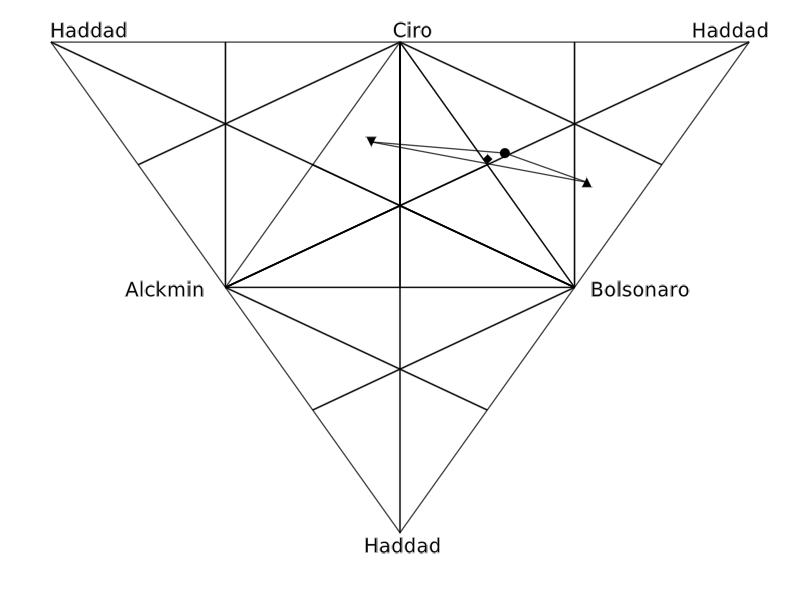
\includegraphics[width=0.8\columnwidth,
height=0.3\textheight]{./images/opened_tetrahedron1.png}
 \caption{Saari's opened tetrahedron }
 \label{fig:ot}
\end{figure}

In what precise percentage of the cases would a candidate have beaten another?
Note that by opening the tetrahedron, the information provided by the volume of
the subregions of the procedure hull is lost\footnote{Moreover, there can be
  some deformations in my implementation of Figure~\ref{fig:ot}. The ensuing
  percentage computations, however, are exact.}. Nevertheless, algebraic
manipulation of the equations in Table \ref{tbl:ws} allows us to answer this
question. Table \ref{tbl:ctn} presents the percentage of scenarios in which this
would have happened. It implies a more complex picture of what happened.
Bolsonaro was the CW, was tied with Ciro as a BW and would have won against Ciro
in roughly 47\(\%\) of the positional voting methods. Nevertheless, it shows
that there were scenarios in which he would have lost to the more inclusive
candidates, Ciro and Alckmin. In Alckmin's case, this could have happened in
surprising \(30\%\) of the cases. However, Ciro could have beaten him in most,
\(\approx 53\%\), of the positional voting methods. Surprisingly, Haddad, who
went to the second round with Bolsonaro, would never have beaten him. The
explanation for that is the following: as shown in Figure \ref{fig:counts},
Haddad and Bolsonaro were both divisive candidates, but Bolsonaro had more
support than Haddad. They were not equally supported/rejected. Given that they
were both divisive, most of their support was in the top choice, they would have
fared equally well or badly under the same positional voting methods, but since
Bolsonaro had more first votes and was less frequently in the bottom of the
rankings than Haddad he actually ``positionally dominated'' Haddad. The same
logic applies to another surprising result: Alckmin would never have beaten
Ciro.

\begin{table}[H]
  \centering
  \begin{tabular}{rrrrr}
    \hline
     & Alckmin & Bolsonaro & Ciro & Haddad \\
    \hline
    Alckmin & 0.0 & 0.31 & 0.0 & 0.58 \\
    Bolsonaro & 0.69 & 0.0 & 0.47 & 1.0 \\
    Ciro & 1.0 & 0.53 & 0.0 & 0.81 \\
    Haddad & 0.42 & 0.0 & 0.19 & 0.0 \\\hline\hline
  \end{tabular}
  % \caption{Proportion of victories in the positional voting procedure set}
  \label{tbl:ctn}
\end{table}


Naturally, proportions do not show what were the decision procedures in which,
for instance, Ciro would have beaten Bolsonaro. Intuitively, voting procedures
that emphasize rejection or more of the middle region of the rankings should
give an advantage to inclusive candidates, which is qualitatively confirmed by
Figure~\ref{fig:ot}. Since the positional voting methods with four candidates
are determined by their \(s_{1}\) and \(s_{2}\) weights, we can visualize all
scenarios by varying them, as in Figure~\ref{fig:positional4c}. It shows the
scenarios Bolsonaro \(\times\) Ciro, Ciro \(\times \) Haddad, and Alckmin
\(\times\) Bolsonaro. Note that, as expected, the only way Alckmin could have
beaten Bolsonaro would be if \(s_{1}\) and \(s_{2}\) were above 0.6. Remember
that when both are 1, the voting procedure is antiplurality, a method equivalent
to saying which candidate voters dislike. However, this universe of cases was
dominated by Ciro, who would have beaten Bolsonaro in any combination of
\(s_{1}\) and \(s_{2}\) higher than the line connecting the points
\((0.51,0.51)\) and \((0.9,0)\). The plot also shows what combinations of
weights lead to \(81\%\) of Ciro \(>\) Haddad: any combination to the right of
the line segment connecting \((0.35,0.35)\) and \((0.55,0.0)\).

\begin{figure}[!h] \centering 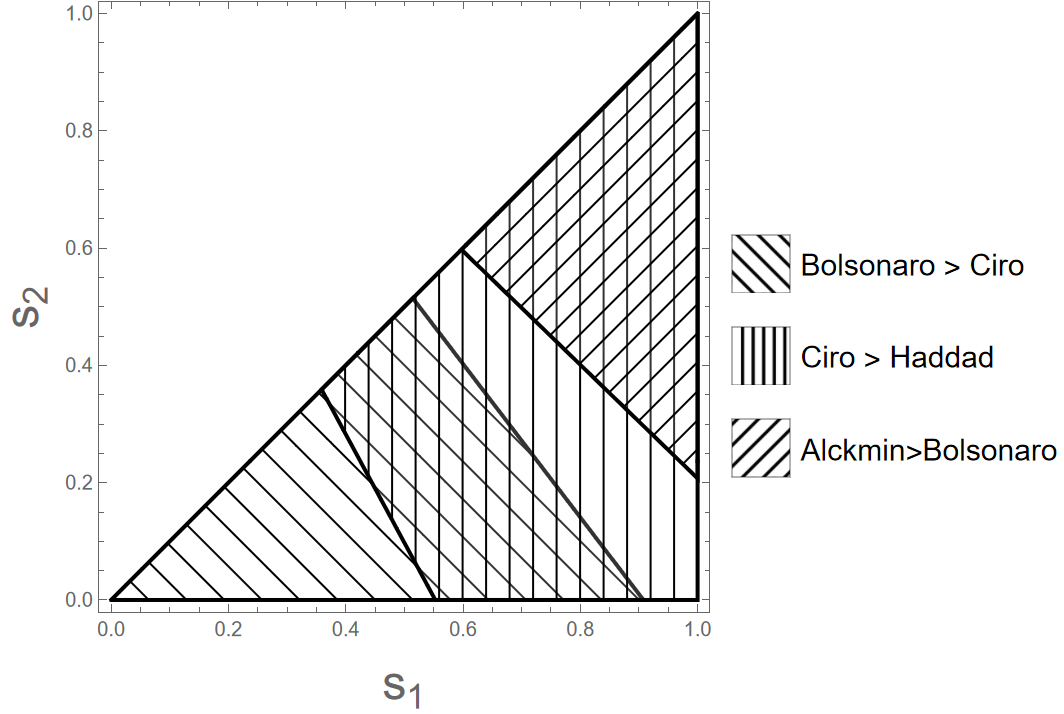
\includegraphics[width=\columnwidth,
height=0.3\textheight]{./images/counterfactual_triangle.png}
\caption{Victory in terms of values of \(s_{1}\) and \(s_{2}\)}
 \label{fig:positional4c}
\end{figure}


Nonetheless, the family of positional voting methods is not, in general,
Independent of the Alternative Set \parencite{kaminski2015empirical}. If we drop
or add candidates, the ``social'' ranking might change without respecting the
ordering of the baseline set of alternatives. Consider the Borda-induced social
ranking in this case: Ciro \( \sim \) Bolsonaro > Haddad > Alckmin. If by
dropping Alckmin, the ranking changes to Bolsonaro > Haddad > Ciro > Alckmin,
then the Borda Count, in this case, would be inducing a ``paradoxical'' result.
In Figure ~\ref{fig:c1dropping}, I consider alternative scenarios by dropping
one of the top 4 candidates.

The positional voting procedures are eminently well-behaved when dropping
candidates from this dataset. There is a minor tilt toward Bolsonaro winning
with the Borda Count in Figure~\ref{fig:notah1}, but as I have previously
argued, this seems like a tie, given the underlying uncertainty. Notice that in
all scenarios where Bolsonaro is still in the alternative set, he would have
been the plurality winner. However, he would have tied with Ciro under Borda and
lost against him with decision procedures that put more weight on rejection, as
in the 4 candidates analysis. In the scenario Ciro was not in the set, Bolsonaro
would again only have lost against Alckmin, but in a minority of cases.


   \begin{figure}[!h] \centering
        \begin{subfigure}[b]{0.475\textwidth} \centering
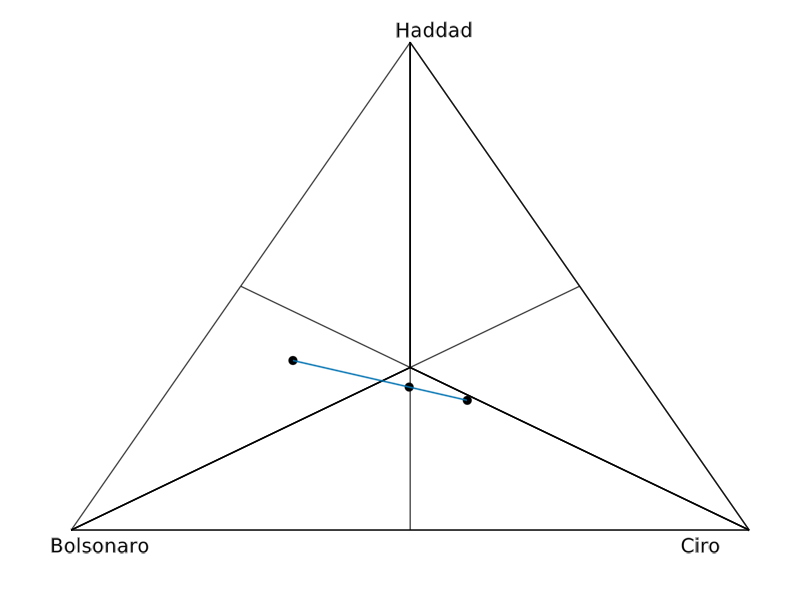
\includegraphics[width=\textwidth]{./images/cw1_nota.png}
             \caption{}% % {{\small Network 1}}
            \label{fig:notac1}
        \end{subfigure} \hfill
        \begin{subfigure}[b]{0.475\textwidth} \centering
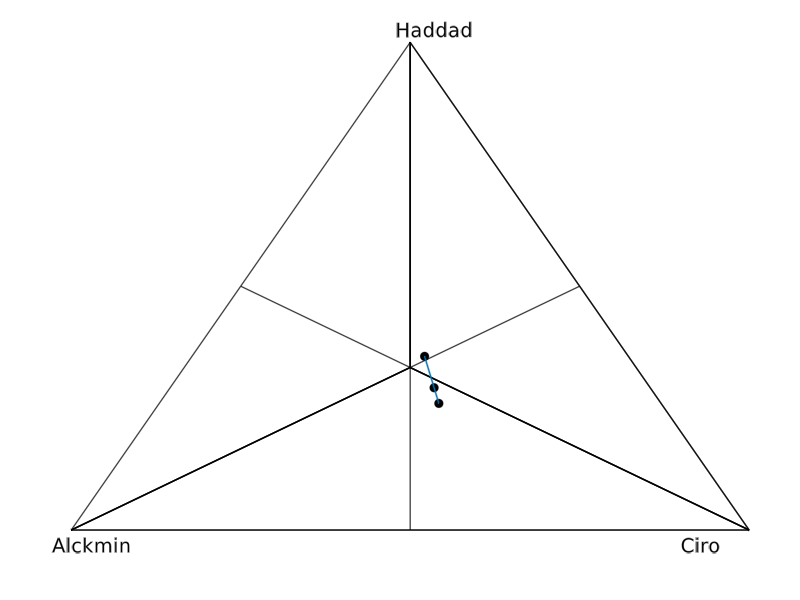
\includegraphics[width=\textwidth]{./images/cw1_notb.png}
             \caption{}% % {{\small Network 2}}
            \label{fig:notbc1}
        \end{subfigure} \vskip\baselineskip
        \begin{subfigure}[b]{0.475\textwidth} \centering
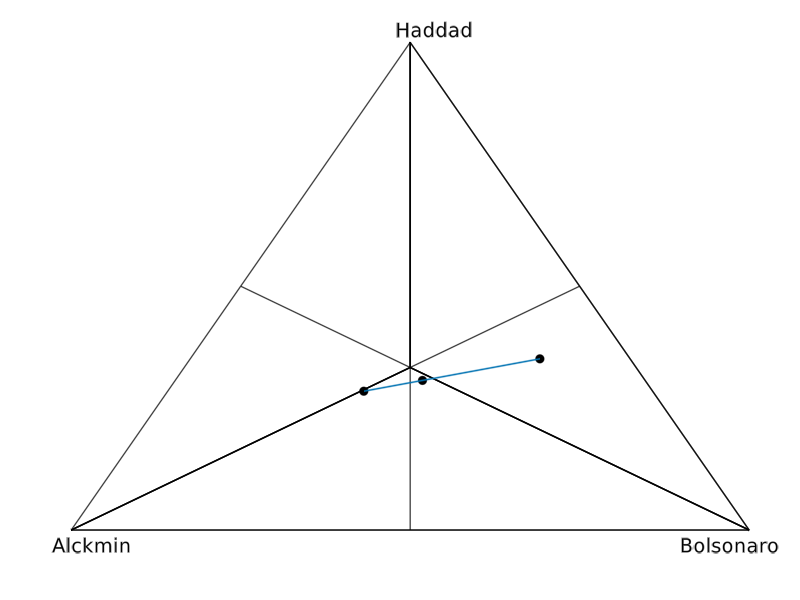
\includegraphics[width=\textwidth]{./images/cw1_notc.png}
            \caption{}%
            \label{fig:notcc1}
        \end{subfigure} \hfill
        \begin{subfigure}[b]{0.475\textwidth} \centering
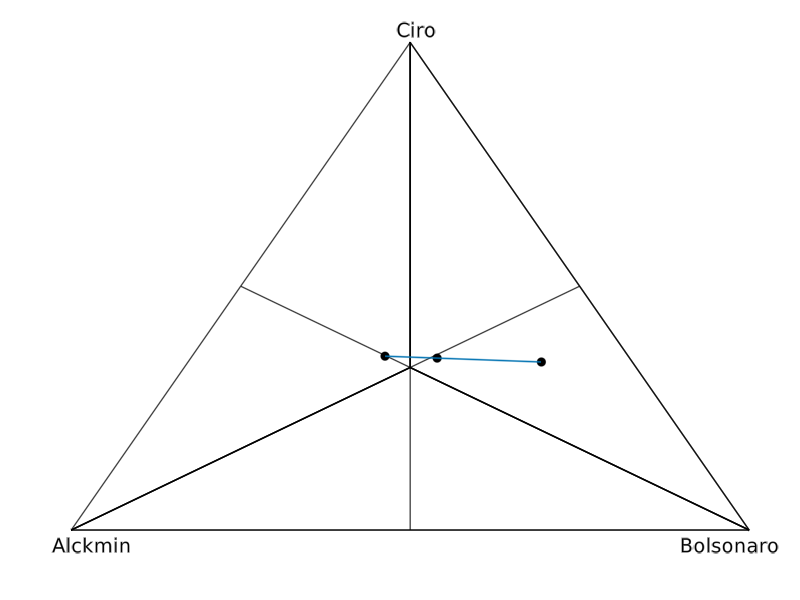
\includegraphics[width=\textwidth]{./images/cw1_noth.png}
             \caption{}% % {{\small Network 4}}
            \label{fig:notah1}
        \end{subfigure}
        \caption[ Positional results when dropping one candidate ] {\small
Positional results after dropping one candidate }
        \label{fig:c1dropping}
    \end{figure}

    We have seen that besides having a high marginal mandate, Bolsonaro was also
    a CW. His victory, thus, was not a fluke or an artifact of institutional
    technology. Neither was he the candidate with the most positional mandate.
    This result revisits the Borda \(\times\) Condorcet controversy. On the one
    hand, he was the CW, the primary normative benchmark for a voting procedure.
    On the other hand, in the Brazilian case, the Borda count would have been a
    more substantial barrier against a divisive candidate. Even though we could
    expect divisive candidates to have fared worse under informationally richer
    decision procedures, a divisive candidate can still be a CW with \(47\%\)
    positional stability/mandate. Yes, Ciro would have won against him in
    \(53\%\) of the positional methods, and at least would have tied with him in
    the Borda count, but most of the methods within this \(53\%\) emphasize
    rejection, and to give more weight to rejection vis-\`a-vis approval seems
    unreasonable under any set of normative expectations demanded of a decision
    procedure for large-scale democratic elections. Due to its symmetry, the
    Borda Count lies at a threshold: its constant decrease in assigning weights
    to the positions in the rankings guarantees that approval matters more than
    rejection, but without throwing away the rejection information. Therefore,
    highly polarized scenarios can lead to the election of a divisive candidate,
    which puts in dispute two reasonable metrics of support: being a CW vs.
    being a BW. This means the paper only gives partial support to the
    hypothesis that informationally richer decision procedures would be enough
    to contain divisive candidates, and two reasonable generalizations of the
    majoritarian credo end up in conflict.

    However, Figure~\ref{fig:notbc1} presents an interesting scenario. Here,
there is no conflict between the perspectives: under both positional and
pairwise perspectives on a mandate, Haddad going to the second round was purely
an institutional fluke. Even though it looks like Haddad would be a plurality
winner if we dropped Bolsonaro, the plurality point is close to a tie with Ciro,
and could be read as such, given the uncertainty. Ciro, thus, now would have
almost 100\(\%\) positional mandate. Moreover, in Table \ref{tbl:margins} it was
shown that Ciro would have beaten him with a majority pairwise comparison, which
gives credence to affirming that Ciro would have won under a majority with
run-off system. In this scenario, the most inclusive candidate would have been
elected. Ceteris paribus, it seems the only way an agreement between the
Borda and Condorcet criteria could be guaranteed to exist in the Brazilian 2018
case would be if Bolsonaro had never been able to run. In this scenario, the
Condorcet Loser would again be beaten, but now a candidate with a solid mandate,
as endorsed both by the pairwise majority comparisons and the entire hull of
positional methods would have been elected.

\section{Conclusion}

The paper contributes to the analysis of the institutional robustness of
polyarchical systems by considering credible alternative voting procedures
outcomes and properties at a critical juncture in Brazil's political history.
First, I argued that the notions of pairwise and positional mandate can be
derived from well-established axiological perspectives to evaluate whether an
electoral result is solely an institutional fortuity. Then, I demonstrated that
even though the aggregation procedure boosted Bolsonaro's victory, it was not
merely its effect, contrary to established theoretical expectations, but neither
was he an undisputed winner under both aforementioned evaluative criteria for
gauging the mandate of a candidate in democratic collective choice situations.

In terms of future research, contrasting Haddad with Lula and analyzing the
effect of the knife attack should provide a more comprehensive picture of what
happened in 2018. Moreover, the pipeline for the analysis is highly
reproducible. Similar work can be done to surveys that contain pairwise
comparisons between the top candidates, as many in Brazil do. As such, any other
majoritarian election in Brazil could be analogously analyzed.
Figure~\ref{fig:notbc1} could also be the starting point for an investigation of
the selection of the pool of candidates allowed to compete for the Executive,
particularly in transitional democracies, given Brazil's lax transitional
justice, and Bolsonaro's intimate connection with the remnants of the Old
Regime. First, from a positive point of view as a causal pathway for democratic
backsliding \parencite{svolik2008authoritarian, nalepa2022after}. Second, from a
normative perspective. What, if anything, justifies restricting classes of
actors from running for certain positions? What values would conflict here?

The most glaring limitation of that paper is that I used only one variable from
the dataset, pairwise comparisons, to simulate alternative scenarios. However,
socio-demographic variables from the dataset could have been used to strengthen
the data imputation procedure. Moreover, roughly less than half of the dataset
is constituted of incomplete pairwise comparisons, and there may be valuable
information on the agent's preferences contained in patterns of missingness.

Another limitation is that agents adapt to new institutional environments. I am
ignoring strategic voting by assuming a direct translation between preferences
and behavior. However, the percentage of strategic voting in a large-scale
election is an open empirical problem
\parencite{straeten10_strat_sincer_heuris_votin_under,kawai2013inferring}.
Nevertheless, a combination of game-theoretic models with a simulation
parameterized by the inferred ranking distribution is a route of research that
could be pursued.

Though I have analyzed the four top candidates, there can be discrepancies when
we have a subset of the alternatives vs. when we have the whole set of
candidates \parencite{saari2001chaotic, kaminski2015empirical}. It is
well-known, for instance, that the Borda Count is susceptible to the
winner-turns-loser paradox. Finally, even though I have analyzed scenarios in
which candidates were removed, it would have been more realistic to simulate the
formation of coalitions and how voters would have reacted to that \parencite
{kaminski1998revival}. The assumption of a pure additive transfer of votes,
implicit when we removed candidates, is not necessarily valid with coalitions,
insofar voters of a center-left candidate, for instance, could vote for the
center-right candidate if they are alienated by an alliance with the Left,
which, in the case of the election under scrutiny, was highly rejected.
\printbibliography





\end{document}
